\chapter{\IfLanguageName{dutch}{Stand van zaken}{State of the art}}%
\label{ch:stand-van-zaken}

% Tip: Begin elk hoofdstuk met een paragraaf inleiding die beschrijft hoe
% dit hoofdstuk past binnen het geheel van de bachelorproef. Geef in het
% bijzonder aan wat de link is met het vorige en volgende hoofdstuk.

% Pas na deze inleidende paragraaf komt de eerste sectiehoofding.

%Dit hoofdstuk bevat je literatuurstudie. De inhoud gaat verder op de inleiding, maar zal het onderwerp van de bachelorproef *diepgaand* uitspitten. De bedoeling is dat de lezer na lezing van dit hoofdstuk helemaal op de hoogte is van de huidige stand van zaken (state-of-the-art) in het onderzoeksdomein. Iemand die niet vertrouwd is met het onderwerp, weet nu voldoende om de rest van het verhaal te kunnen volgen, zonder dat die er nog andere informatie moet over opzoeken \autocite{Pollefliet2011}.
%
%Je verwijst bij elke bewering die je doet, vakterm die je introduceert, enz.\ naar je bronnen. In \LaTeX{} kan dat met het commando \texttt{$\backslash${textcite\{\}}} of \texttt{$\backslash${autocite\{\}}}. Als argument van het commando geef je de ``sleutel'' van een ``record'' in een bibliografische databank in het Bib\LaTeX{}-formaat (een tekstbestand). Als je expliciet naar de auteur verwijst in de zin, gebruik je \texttt{$\backslash${}textcite\{\}}.
%Soms wil je de auteur niet expliciet vernoemen, dan gebruik je \texttt{$\backslash${}autocite\{\}}. In de volgende paragraaf een voorbeeld van elk.
%
%\textcite{Knuth1998} schreef een van de standaardwerken over sorteer- en zoekalgoritmen. Experten zijn het erover eens dat cloud computing een interessante opportuniteit vormen, zowel voor gebruikers als voor dienstverleners op vlak van informatietechnologie~\autocite{Creeger2009}.

In dit gedeelte van de scriptie zal de huidige manier van asset tracking binnen de bouwindustrie beschreven worden. Dit houdt in een uitgebreide beschrijving van de reeds gebruikte technologieën voor asset tracking in het algemeen en specifiek op een bouwwerf. Bluetooth Low Energy hoort hier ook bij en de werking ervan zal dus ook uitvoerig worden besproken, samen met de verschillen tussen BLE en het klassieke Bluetooth. Verder zal er verklaard worden hoe Bluetooth Low Energy bij smartphones werkt. Beveiliging van asset tracking technologieën wordt in dit deel van de scriptie ook uitvoerig besproken. De focus zal op Bluetooth Low Energy liggen maar de andere technologieën zullen ook besproken worden.

\subsection{Asset tracking in de bouwindustrie}

Het lokaliseren van middelen op een bouwterrein is in het verleden steeds een uitdagende taak geweest. Onbenutte middelen zoals werkgereedschap of machines zouden tot de grote meerderheid van verspilling in de bouwindustrie bijdragen \autocite{Nasr2013}. Door het gebruik van verschillende technologieën hebben onderzoekers zich gericht tot het ontwikkelen van plaatsbepalingssystemen als poging om dit probleem aan te pakken. Met behulp van deze systemen kan activa zoals werkgereedschap, machines of personeel gevolgd worden met onder andere als doel op deze manier hun veiligheid te bewaren.\\

De technologieën die het meest gebruikt worden voor asset tracking in de bouwindustrie zijn GPS, RFID en UWB. Er zijn nog andere technologieën, namelijk barcode en QR code, die gebruikt worden voor asset tracking maar niet specifiek in de bouwindustrie. Deze zullen ook uitgebreid beschreven en later vergeleken worden met de andere technologieën aangezien het onderzoek in deze scriptie niks uitsluit.

\subsubsection{Global Positioning System}

Het Global Positioning System (GPS) is een positionering en navigatie systeem ontwikkeld door het Amerikaans ministerie van defensie \autocite{McNeff} in de jaren zestig. Het bestaat ondertussen uit meer dan dertig satellieten die rond onze aarde cirkelen. Deze kunnen met behulp van de atomische klok, die elke satelliet aan boord heeft, en hun gekende precieze locatie continu uitzenden door middle van signalen die gebruikers op aarde kunnen ontvangen. Hiermee is het mogelijk de tijd en locatie van de gebruiker te bepalen met respectievelijk een paar nanoseconden en meter speling. Elke GPS-satelliet kent zijn eigen baanlocatie en systeemtijd. Om de positie van een ontvanger nauwkeurig te kunnen bepalen, moeten er ten allen tijde minstens vier satellieten zichtbaar zijn die voldoende van elkaar gescheiden zijn. Met behulp van trilateratie, wat de basis is van de gebruikte technieken waarbij de afstandsmetingen van \(n + 1\) satellieten worden gebruikt voor een n-dimensionale positiebepaling \autocite{Rahman2012}, is het mogelijk de positie te bepalen van een gebruiker op aarde. Hier zal niet verder op uitgebreid worden, aangezien dit niet aansluit bij het doel van deze scriptie.\\

%TODO: Praten over hoe dit in de bouwindustrie werkt + FIGUURTJES
Vandaag de dag is GPS de meest gebruikte technologie voor het traceren van activa \autocite{Nasr2013}. In de bouwindustrie is GPS zeer handig door zijn groot werkbereik. Hierdoor kunnen bedrijven hun activa volgen over de hele wereld. Dit wordt gerealiseerd aan de hand van trackers die geïnstalleerd worden op het dashboard van voertuigen en machines of op een andere veilige plek waar de tracker niet makkelijk beschadigd kan worden. Deze trackers zijn aangekocht bij een bepaald bedrijf die meestal een bijhorende website of software voorziet waar de klant kan inloggen om de locatie van al zijn activa te raadplegen. Soms voorzien deze GPS trackers extra functionaliteiten zoals diagnostische informatie over de motor \autocite{Devlin2009}, wat zaken inhoudt als stationair draaien, hard remmen, kilometers per liter, etc.

\subsubsection{Radio Frequenty Identifier}

Radio Frequenty Identifier (RFID) is een draadloze communicatietechnologie die in zijn simpelste vorm objecten kan detecteren, opsporen, identificeren, volgen en controleren \autocite{Tan2022}. Het bestaat voornamelijk uit drie elementen: readers (figuur \ref{fig:rfidhandheld}), antennes en tags (figuur \ref{fig:rfidtag}). De reader, soms ook transeiver genaamd, heeft de mogelijkheid radio frequentie (RF) elektrische golven te sturen naar een of meerdere RFID tags. De tags hoeven dus niet in het gezichtsveld van de reader te zitten. Deze tags, actief of passief, ontvangen de elektrische golf met hun antenne en zetten deze met behulp van een spoel om naar elektrische stroom. Vervolgens wordt deze stroom door de tag, die bevestigd is aan een fysiek object, gebruikt om terug via een RF elektrische golf een antwoord te sturen naar de reader.\\

RFID tags kunnen opgedeeld worden in drie soorten. Actieve, semi-passief en passieve tags \autocite{Mezzanotte2021}.  Actieve tags bezitten een batterij die heel het systeem van stroom voorziet. Zo een systeem (van een actieve tag) bestaat uit een ontvanger, een zender en omgevingssensoren. Het principe van een passieve tag is vrij verschillend, want deze tags zullen de stroom, die toekomt als RF elektrische golf omgezet wordt door de ingebouwde spoel, gebruiken om een antwoord te verzenden. Passieve tags hebben geen batterij en transmitter. Semi-passieve tags zijn een mix van actief en passief, in de zin dat ze dezelfde functioneringsprincipe gebruiken, maar ze hebben wel een batterij om de microchip of sensoren van stroom te voorzien.\\

\begin{figure}
    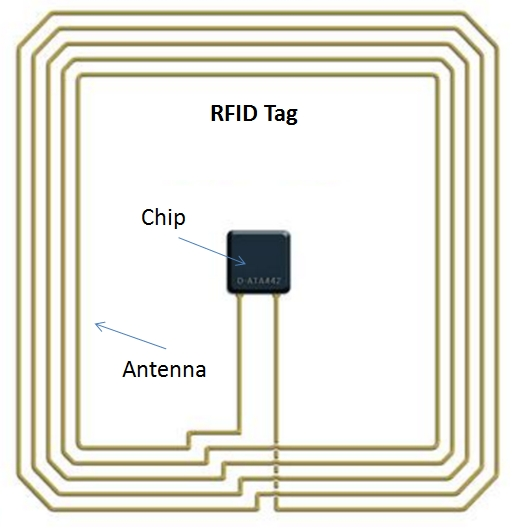
\includegraphics[width=\linewidth]{RFID.jpg}
    \caption{RFID tag}
    \label{fig:rfidtag}
\end{figure}

\begin{figure}
    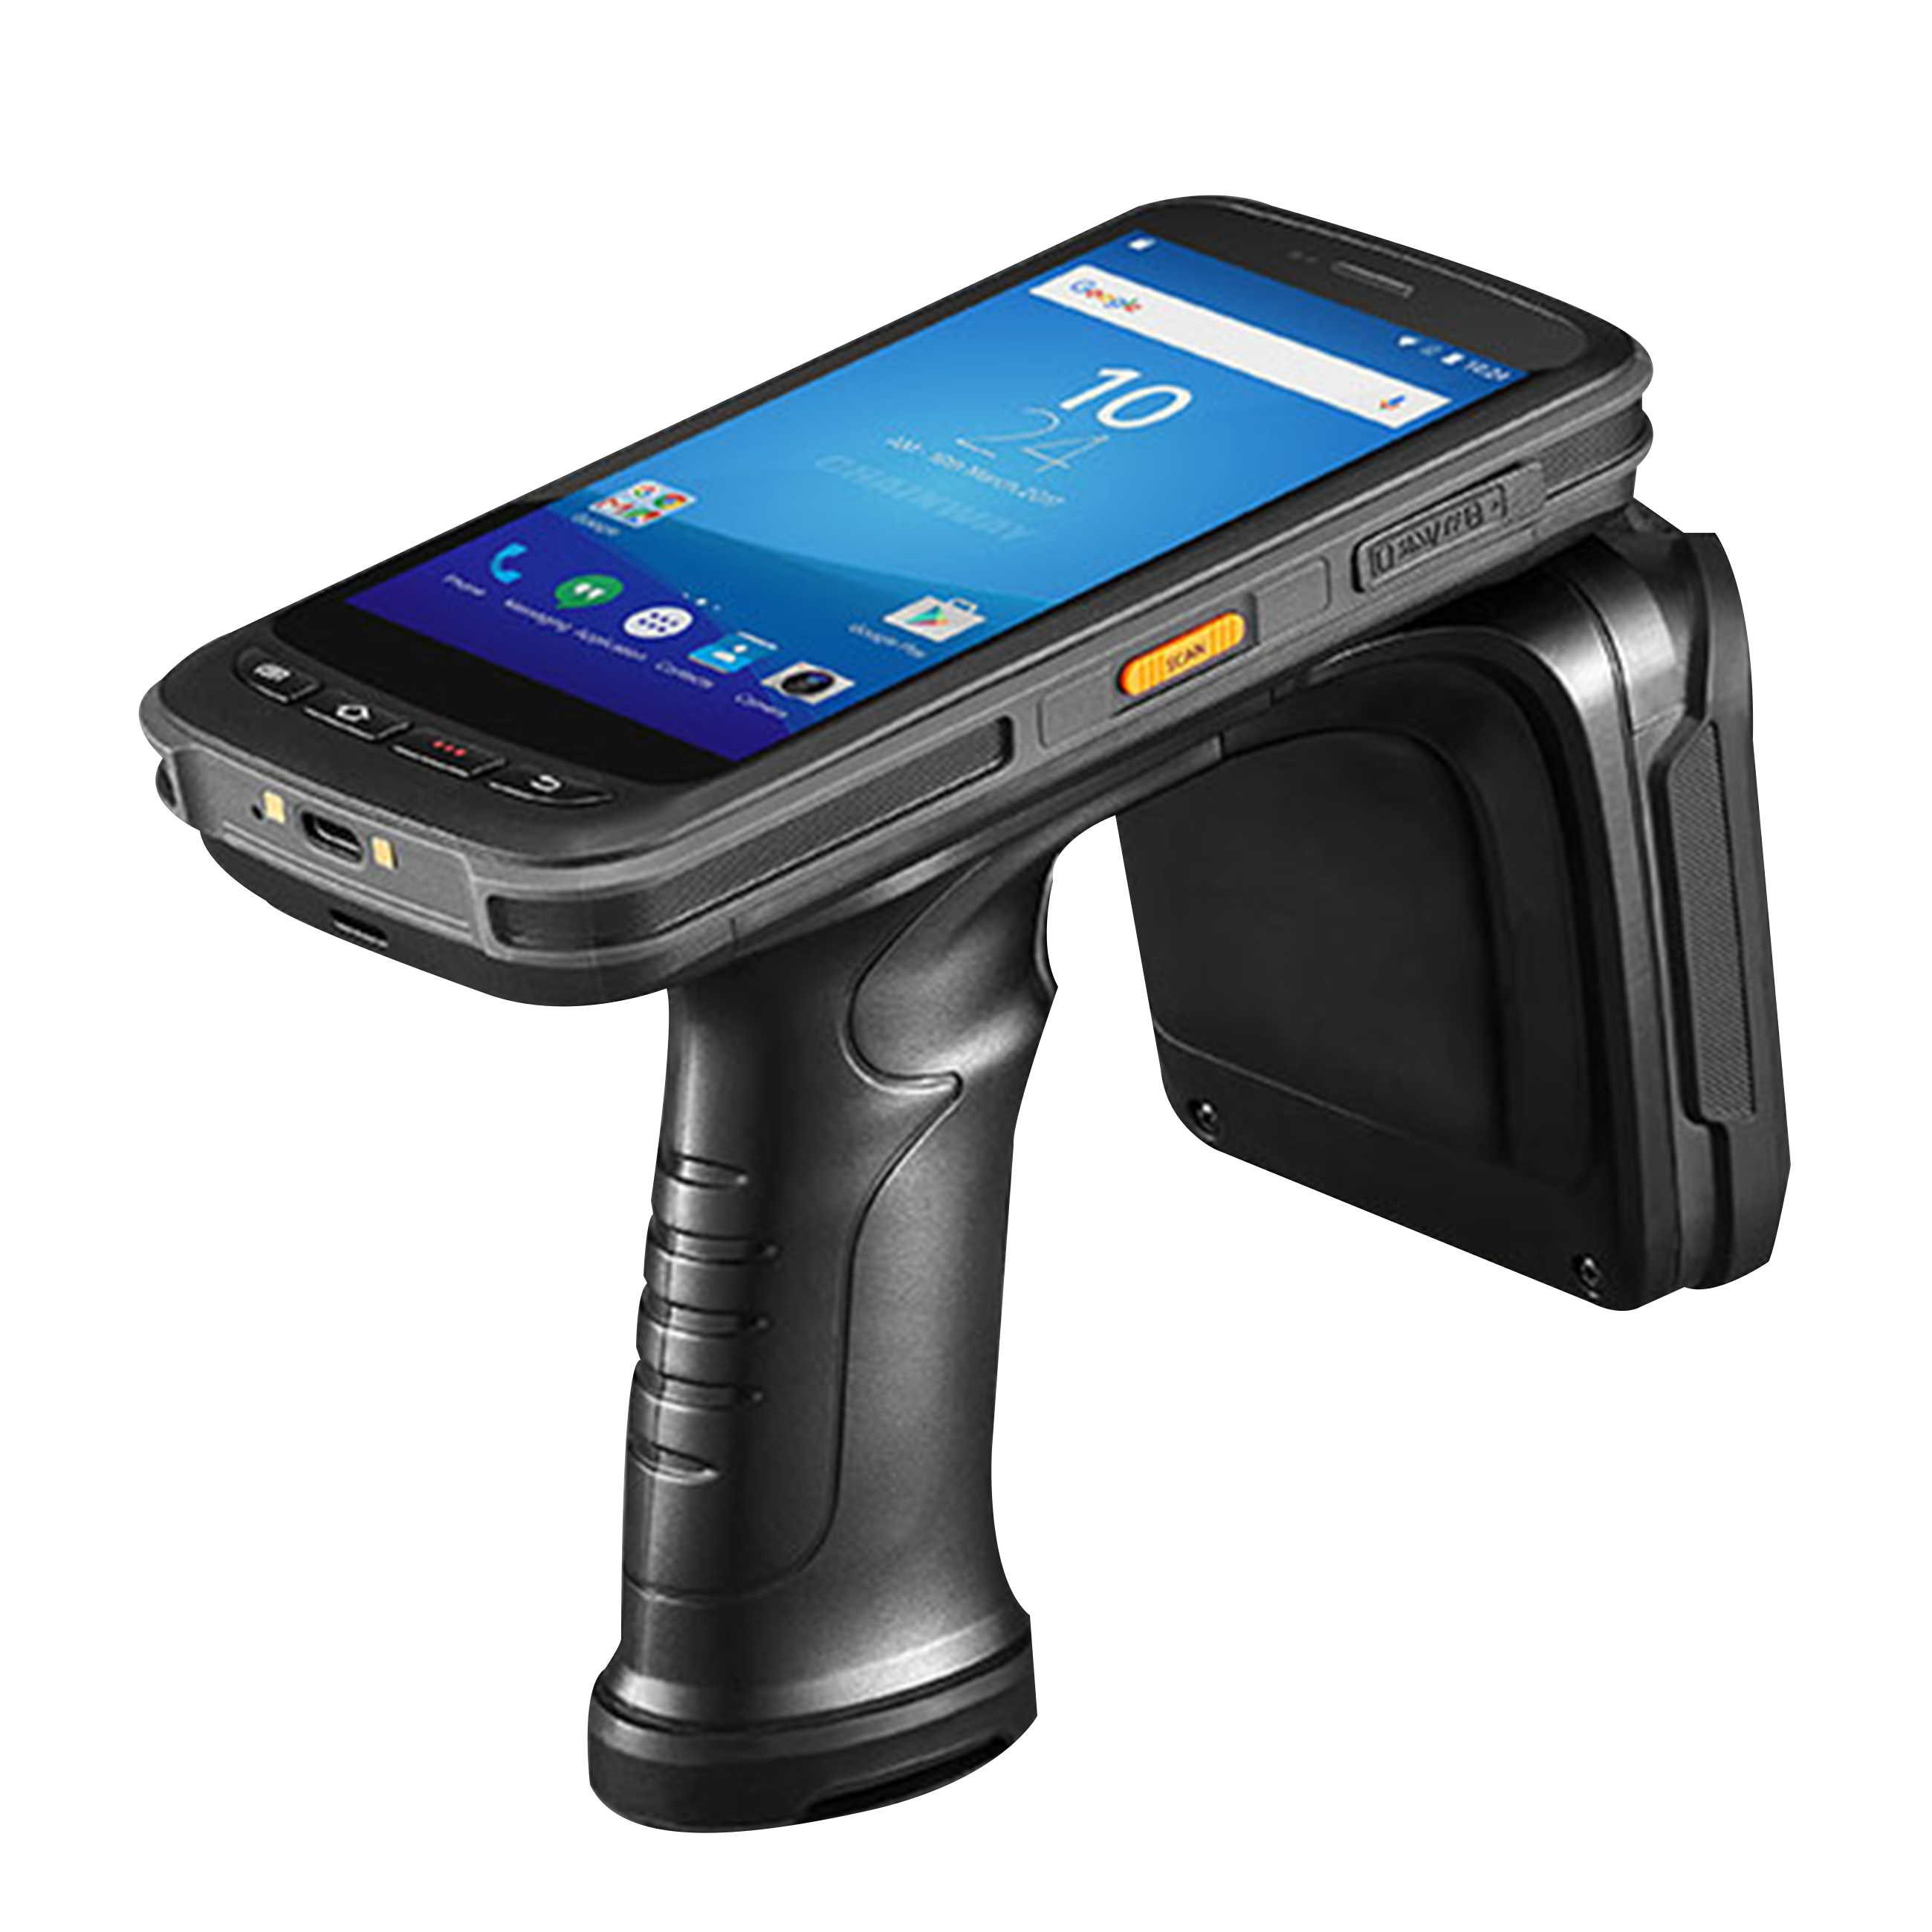
\includegraphics[width=\linewidth]{handheld.png}
    \caption{RFID handheld}
    \label{fig:rfidhandheld}
\end{figure}

%TODO: \autocite{Roberts2006} <-- NOG GEBRUIKEN ERGENS EN VOOR FIGUURTJES\\

RFID wordt vaak gebruikt in sectoren waar er bijvoorbeeld producten worden gestockeerd in een magazijn. Indien er door een reader een vraagimpuls wordt verzonden, kunnen de tags antwoorden met een digitaal gegeven. Dit is vaak hun identificatienummer. Op deze manier kan een ID worden toegewezen aan ieder product bij het printen van de tag en kan een magazijnmedewerker met behulp van een reader op deze manier het juiste product vinden in een magazijn.\\

In de bouwindustrie wordt dit op een gelijkaardige manier gebruikt om assets te traceren en lokaliseren.\\

%TODO: Verder uitwerken

\subsubsection{Ultra-wideband}

Ultra-wideband is een draadloze radiotechnologie die ontwikkeld is om over een korte afstand met een hoge snelheid gegevens over te brengen \autocite{Rahayu2008}. Door zijn hoge bandbreedte is UWB geschikt voor verschillende doeleinden zoals video en audio maar ook in traditionele toepassingen zoals niet-coöperatieve radarbeeldvorming en andere zaken zoals het verzamelen van nauwkeurige plaatsbepalingen en tracking. Een perfecte implementatie werd hiervan gedaan door Apple die UWB gebruikt als technologie voor de Apple AirTag \autocite{Griffith2021}.\\

 Het is mogelijk voor UWB apparaten, door passende technische normen, om te opereren in het spectrum dat door bestaande radiodiensten bezet worden zonder storing te veroorzaken. Dit heeft als voordeel dat op deze manier schaarse spectrumbronnen efficiënter gebruikt kunnen worden.\\

Ultra-wideband wordt reeds gebruikt om indoor zaken te traceren aangezien dit hiervoor een zeer geschikte technologie is. Met behulp van tags en sensors, een gelijkaardig systeem als BLE en RFID, kunnen assets getraceerd en 2D weergegeven worden \autocite{Siddiqui2019}. Dit wordt gerealiseerd door middel van Angle of Arrival (AOA) en Time of Arrival (TOA) algoritmen te gebruiken die samen met het verschil tussen de verschillende technologieën wat verder in deze scriptie uitgelegd zullen worden.

\subsubsection{Barcode}
Barcodes zijn de meest gebruikte vorm van asset tracking \autocite{Penny2022} en is al in gebruik sinds de jaren zestig. Een barcode is een afbeelding dat bestaat uit een serie zwarte en witte balkjes \autocite{Rankin2020}. Dit visueel patroon kan gelezen worden door een barcode scanner of ook barcode lezer genoemd. Zo een barcode scanner kan aan de hand van een ingebouwde lichtbron en een lens de afbeelding scannen en decoderen, door middel van een vast algoritme, naar iets betekenisvol. Barcodes worden het meest gebruikt in detailhandel, magazijnen, voor inventarisatie en niet te vergeten om kassasystemen van supermarkten te automatiseren. Het is dus zeker mogelijk barcodes te gebruiken als asset tracking technologie in de bouwindustrie, maar of dit daarvoor geschikt is zal later in deze scriptie besproken worden.\\

Er zijn twee soorten barcodes namelijk twee dimensionale, ook wel QR Codes genoemd (figuur \ref{fig:qr}), en eendimensionale barcodes zoals op figuur \ref{fig:bar}.

\begin{figure}
    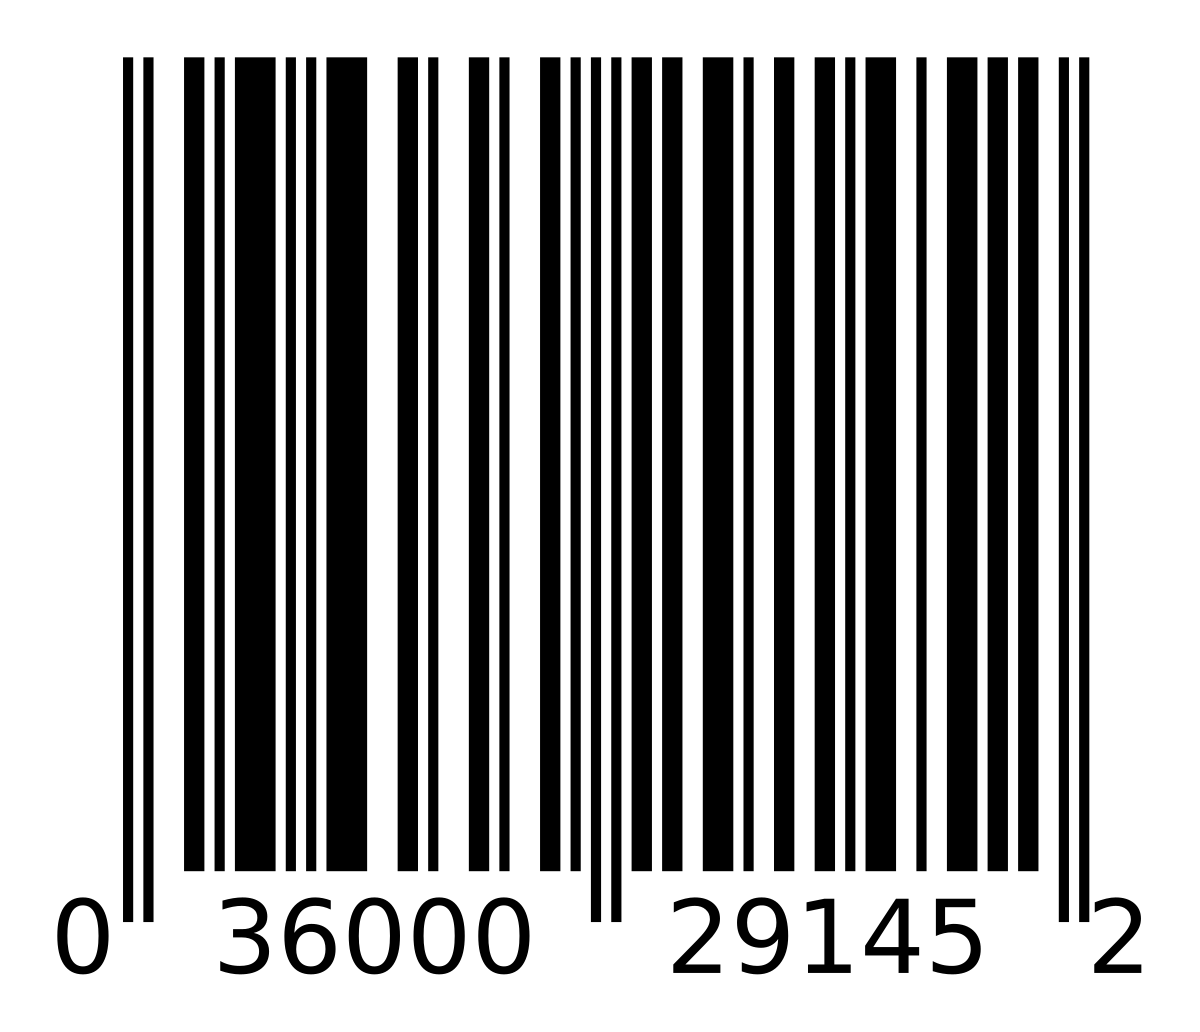
\includegraphics[width=12cm, height=9cm]{barcode.png}
    \caption[Barcode]{Dit is een generieke barcode.}
    \label{fig:bar}
\end{figure}

\begin{figure}
    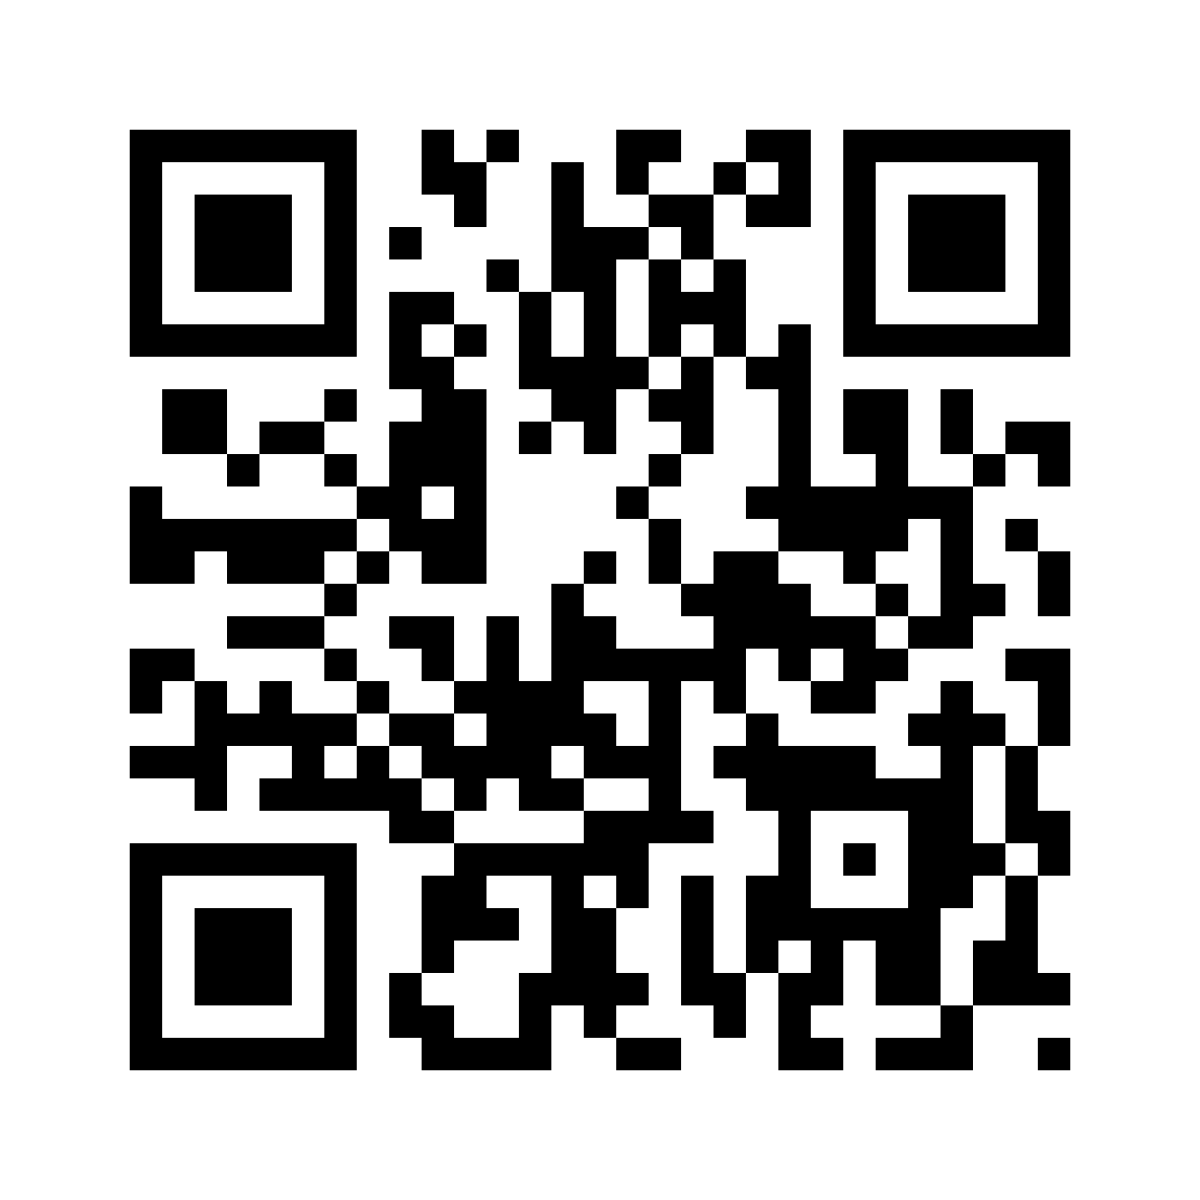
\includegraphics[width=10cm, height=10cm]{QRCode.png}
    \caption[QR Code]{Dit is een generieke QR code.}
    \label{fig:qr}
\end{figure}

\subsubsection{Quick Response codes}
QR codes of zoals eerder vermeld ook bekend als tweedimensionale barcodes zijn ook een soort barcode, zoals de naam al aangeeft, maar meer complex. Ze zijn uitgevonden in 1993 door een Japans automobielbedrijf. Tweedimensionale barcodes kunnen buiten gewoon tekst ook bijvoorbeeld de prijs, voorraadniveaus en zelfs productafbeeldingen opslaan en die informatie dan vrijgeven indien iemand met een compatibel toestel zoals een smartphone de code scant.\\

QR is een afkorting voor quick response. Dit soort code wordt gewoonlijk gebruikt voor marketing doeleinden \autocite{Rodrigue2022} waar ze worden vaak gebruikt om gebruikers om te leiden naar landingspagina's, websites, sociale-mediaprofielen of winkelcoupons. Ze worden de laatste tijd ook vaak gebruikt in hippe restaurants als vervanger van de papieren menukaart. Het ontwerp, de functionaliteit en doeleinden van de QR codes kunnen considerabel verschillen maar deze QR codes vallen meestal in een van de volgende twee categorieën, namelijk statische of dynamische QR codes. \\

Statische QR codes zijn uitstekend voor het opslaan van vaste of gevoelige informatie, zoals identificatienummers van bepaalde zaken of toegangscodes. Dit zou dus ideaal zijn voor bijvoorbeeld identificatienummers van activa die traceerbaar moeten zijn aangezien deze informatie niet regelmatig moet bijgewerkt worden. \\

Dynamische QR codes daarentegen laten toe de scanbare informatie zonder limiet bij te werken. Dit is mogelijk aangezien de informatie niet in de code ingebakken zit, in plaats daarvan leidt de code de persoon die de code scant om naar een specifieke URL die altijd aangepast kan worden. Een mooie toepassing hiervan is de eerder besproken restaurantmenu. \\

De werking van dit soort barcode is net zoals de mogelijke functionaliteiten iets complexer maar nog steeds hetzelfde principe als dat van een normale barcode. Een QR code bestaat uit drie grotere vierkanten en een patroon van zwarte en witte blokjes. Dit patroon is uniek per code en bevat de informatie die door te scannen, wat maar enkele seconden duurt, met een compatibel toestel leesbaar wordt. Zo goed als alle smartphones kunnen QR codes standaard scannen met behulp van de camera app en indien dit niet het geval is zijn er meer dan genoeg apps die dit mogelijk maken. De drie grotere blokjes hebben als functie de oriëntatie van de code weer te geven. Hierdoor kunnen scanners op de correcte manier de code scannen.

\subsection{Bluetooth Low Energy}
Bluetooth Low Energy, ook wel Bluetooth Smart genoemd, is een wireless personal area network (PAN) dat deel uitmaakt van de Bluetooth 4.0 standaard, ontworpen en ontwikkeld door de Bluetooth Special Interest Group (SIG). Dit is het non-profit normalisatie-instituut dat toezicht houdt op de ontwikkeling van Bluetooth standaarden en het beheer van licenties van de Bluetooth-technologieën en -handelsmerken aan fabrikanten. \\

BLE zendt gegevens uit via 40 kanalen in de 2.4GHz ISM-frequentieband \autocite{Kumbhar2017}. Dit is een gedeelte van het radiospectrum, gereserveerd voor industriële (Industrial), wetenschappelijke (Scientific) en medische (Medical) doeleinden zoals microgolven, medische apparatuur, procesverwarming en soorten elektrolampen. De laatste jaren zijn er ook draadloze communicatie toestellen geproduceerd die ook deze banden kunnen gebruiken zonder storing te veroorzaken voor bestaande apparaten die gebruik maken van de ISM-banden, zoals BLE.\\

Vergeleken met Bluetooth Classic, ondersteunt Bluetooth Low Energy meerdere communicatietopologieën, namelijk point-to-point, mesh en broadcast terwijl Bluetooth Classic enkel point-to-point ondersteunt. Door de mesh topologie kunnen er grootschalige en betrouwbare netwerken gebouwd worden tussen verschillende toestellen. Hoewel Bluetooth vroeger meer bekend stond voor het uitwisselen van gegevens tussen toestellen wordt het tegenwoordig ook vaak gebruikt voor het positioneren van apparaten. Dit wordt gedaan aan de hand van een paar concepten.\\

\subsubsection{Real-Time Locating System}

Een Real-Time Locating System heeft als hoofddoel het identificeren en real-time de positie of hoek van bepaalde objecten te kunnen bepalen \autocite{Lehtimaki2018}, in dit geval gebruik makend van radio golven maar nog mogelijkheden zijn infrarood of ultrasound. Dit is meestal in een gebouw of een ander afgebakend gebied. Dit is van toepassing op bijvoorbeeld het bepalen van de locatie van assets of mensen en nog zeer veel IoT (Internet of Things) toepassingen.

\subsubsection{Angle of Arrival}

Bluetooth maakt gebruik van twee verschillende methoden om de locatie, specifiek de afstand en richting van een Bluetooth Low Energy signaal te bepalen. Angle of Arrival is hier een van. 
In deze methode zendt een apparaat, zoals een asset tag met behulp van een antenne een signaal uit. Deze wordt opgevangen door een ontvangend apparaat die over een reeks antennes beschikt. Hierdoor kan de ontvanger gegevens verzamelen, waarmee de richting van het signaal berekend kan worden (zoals te zien is op figuur \ref{fig:aoa}). Theoretisch gezien zullen de ontvangende reeks antennes faseverschillen zien door de verschillende afstanden tot de zender, maar dit is net zoals de meeste zaken in de praktijk niet zo simpel.
\subsubsection{Angle of Departure}

Het fundamentele idee van Angle of Depature is hetzelfde als deze van Angle of Arrival, maar nu zijn de rollen omgedraaid. Het apparaat dat een signaal ontvangt, heeft maar een antenne en hetgeen dat de data verzendt, heeft er meerdere. Dit kan u zien op figuur \ref{fig:aop} waarbij TX de zender is en RX de ontvanger. Bij Angle of Departure berekent het ontvangende apparaat zelf zijn locatie aan de hand van de verschillende antennes van het zendende apparaat en hun posities.\\

\begin{figure}
    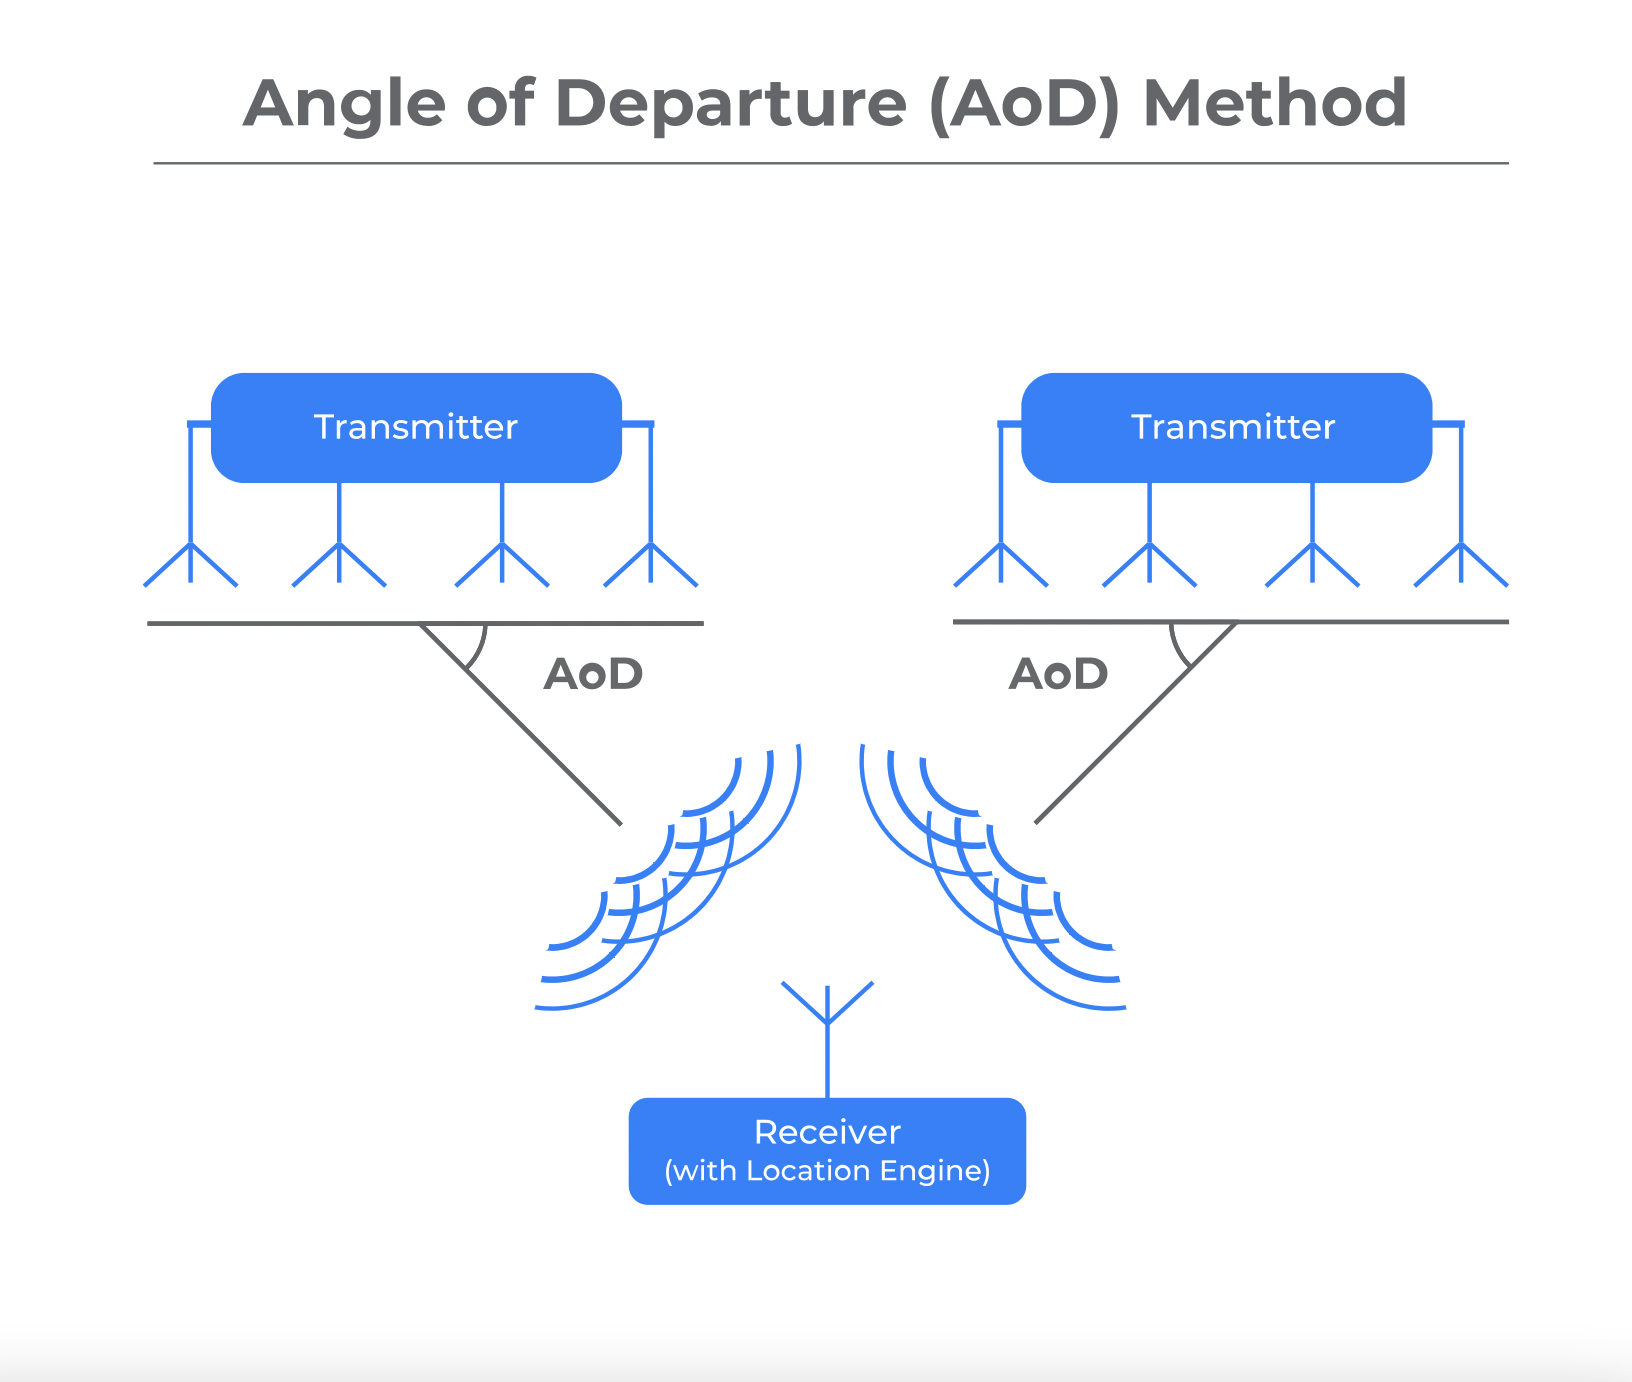
\includegraphics[width=\linewidth]{angle_of_departure_graphic.png}
    \caption{Angle of Departure}
    \label{fig:aop}
\end{figure}

\begin{figure}
    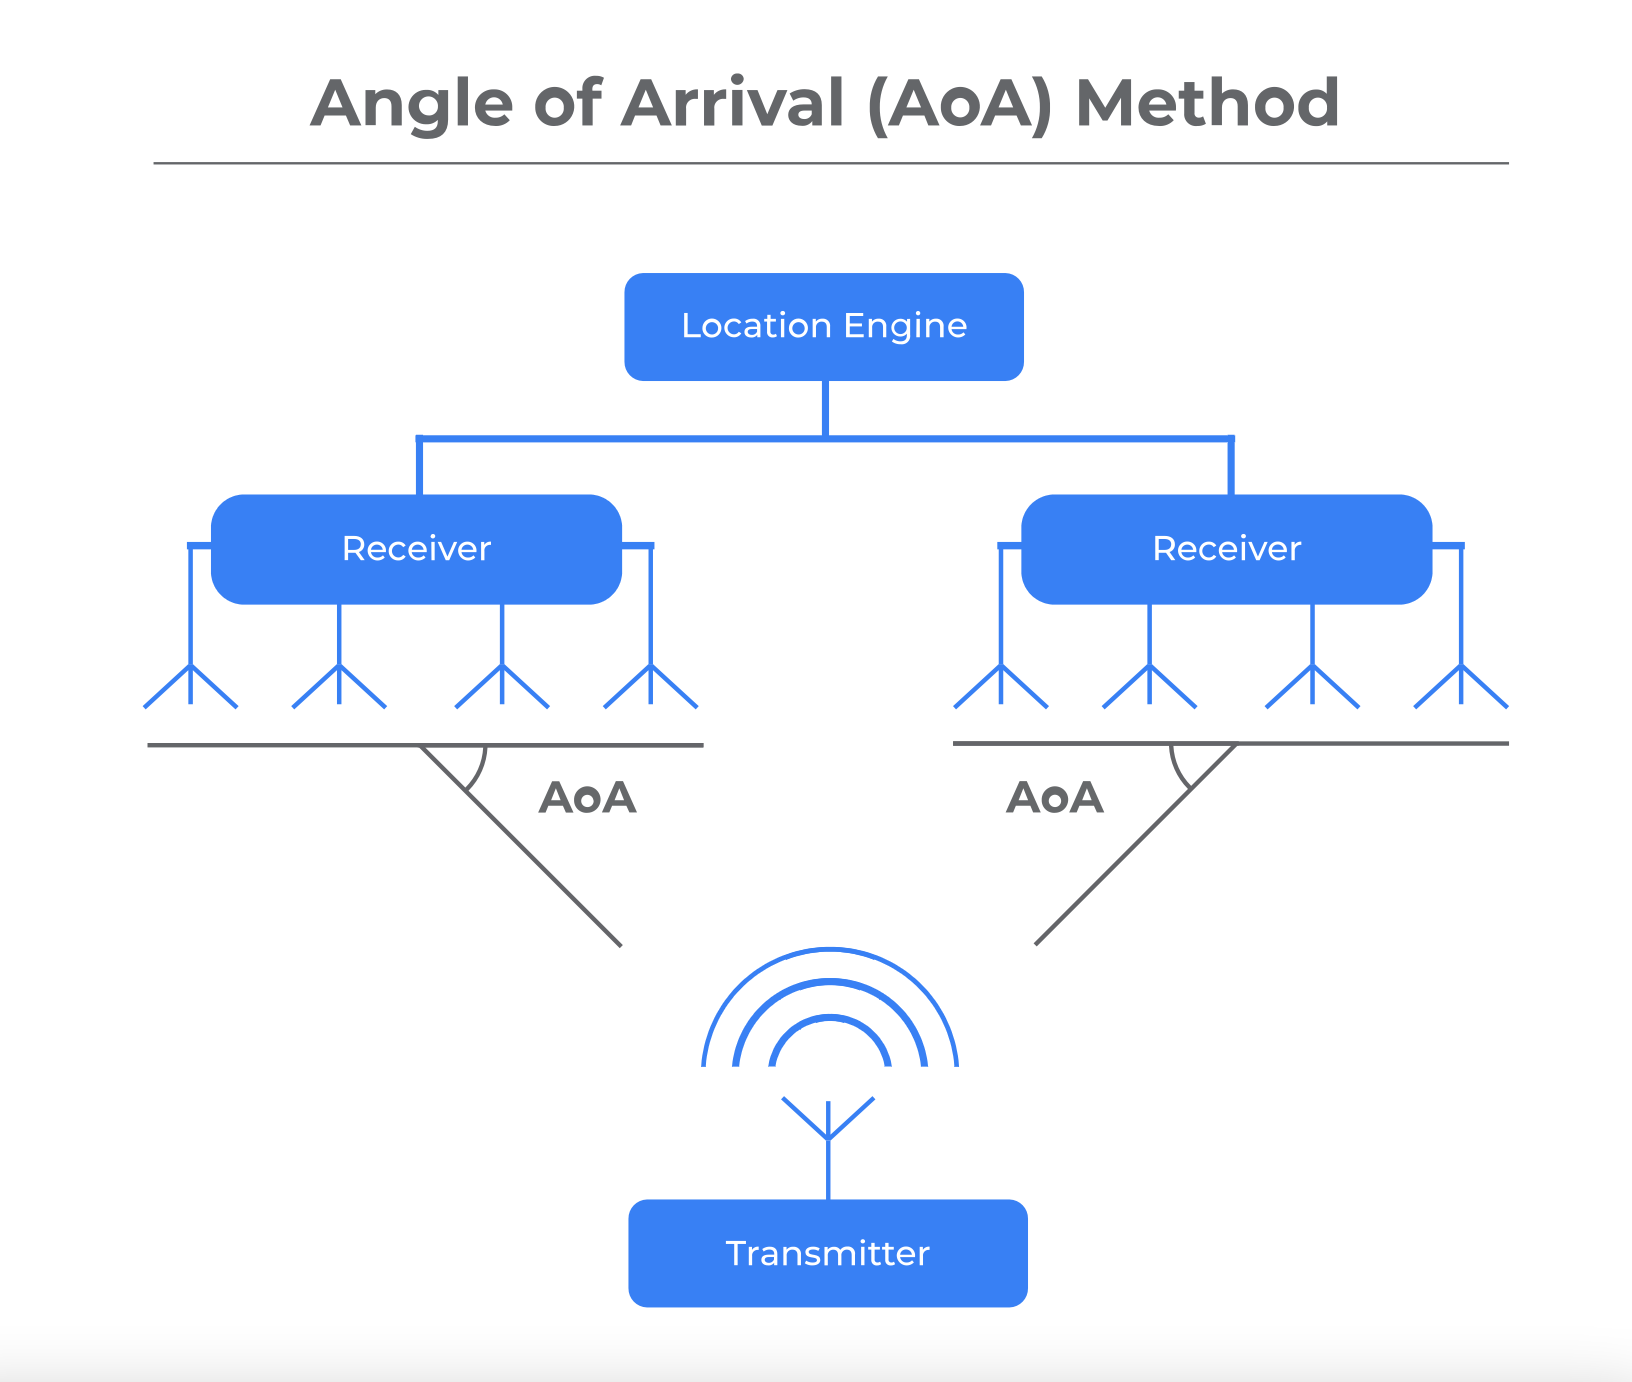
\includegraphics[width=\linewidth]{angle_of_arrival_graphic.png}
    \caption{Angle of Arrival}
    \label{fig:aoa}
\end{figure}

Hier kunnen veel combinaties in gemaakt worden en met behulp van de Received Signal Strength Indicator (RSSI) zijn er nog eens extra mogelijkheden.


%TODO: Verder uitwerken
\subsubsection{Received Signal Strength Indicator}

De Received Signal Strength Indicator (RSSI) geeft het signaalvermogen aan de ontvangende kant weer \autocite{Jais2015} . Dit kan gebruikt worden om de afstand tussen bijvoorbeeld twee apparaten te bepalen.

%sequentie uitgelegd, in wat wordt dit uitgedrukt? toa en andere mss ook uitleggen?

\subsubsection{Security}
Een zeer belangrijke eigenschap van een technologie die waardevolle activa moet kunnen traceren is beveiliging. Hoe veilig is het gebruik van Bluetooth Low Energy voor asset tracking doeleinden nu eigenlijk? Op een bouwwerf staat veel materiaal met enorme waarde zoals machines, voertuigen en ander kostbaar werkmateriaal. Het zou niet interessant zijn als onbevoegden zomaar waardevol materiaal zou kunnen opsporen.\\

Bluetooth Low Energy tags en beacons hebben maar een beperkte functionaliteit. Het enigste verschil tussen de twee is dat tags verplaatsbaar zijn en beacons meestal stationair zijn, maar ze hebben dezelfde functionaliteit namelijk zijn uniek identificatienummer met een vast interval uitzenden via radiofrequentie. Afhankelijk van dit interval kan die tag of beacon dit meerdere jaren doen zonder het vervangen van de batterij. Aangezien dit gebeurd door middel van de reeds eerder besproken broadcast modus \autocite{Sevier2019} kan ieder apparaat die luistert naar Bluetooth Low Energy signalen, door bijvoorbeeld gebruikt te maken van een simpele BLE scanner app van de App of Play Store, dit oppikken. \\

Dit is een nadelige situatie maar onvermijdelijk in het geval van Bluetooth Low Energy aangezien dit nu eenmaal de manier is waarop de Bluetooth protocol opzettelijk ontwerpen is. Indien we kijken naar andere technologieën zoals GPS of RFID zien we wel een verschil.\\

In het geval van RFID kunnen we een gelijkaardige conclusie maken. RFID tags zijn net zoals BLE tags vrij “dom” \autocite{Juels2006}. In de zin dat bij RFID iedereen met een RFID scanner een tag kan scannen en data kan terugkrijgen zonder authenticatie. Dit is een minder groot probleem indien de teruggegeven data, meestal een ID, willekeurig is en geen persoonlijke data meegeeft. Het nadeel hiervan is net zoals bij BLE tags dat iedereen met de juiste apparatuur, in dit geval een RFID scanner, tags kan opsporen en uitlezen.\\

GPS heeft dit probleem niet. Een GPS tracker die gemonteerd zit in een voertuig, op een machine of een ander voorwerp heeft een simkaart. Met behulp van deze kaart kan de GPS tracker zijn locatie en andere data rechtstreeks via het mobiel internet naar de servers sturen van het bedrijf waarvan de trackers aangekocht geweest zijn. Die servers zorgen dan dat de correcte data bij de juiste klanten terechtkomt indien zij inloggen in hun accounts. \\

Barcode en QR code hoeven vermeld te worden op vlak van security aangezien je die eerst manueel moet zoeken voor de code gescand kan worden.

%TODO: encription ble signals

\subsection{Smartphones}
Vandaag de dag zijn zo goed als alle smartphones BLE-compatibel. Dit wil zeggen dat deze probleemloos kunnen communiceren met zaken als smartwatches, headphones, fitness trackers en vooral in het geval van dit onderzoek belangrijk, beacons. Bluetooth Low Energy wordt heel vaak gebruikt voor advertenties te lanceren op smartphones indien een persoon dicht bij een voorwerp loopt. Bijvoorbeeld iemand wandelt voorbij een laptop die net uitgekomen is met de app van die bepaalde winkel geïnstalleerd op zijn smartphone. In dit geval kan een BLE beacon geplaatst zijn in de buurt die continu signalen uitzend over die bepaalde laptop zodat mensen met de app daar reclame over kunnen ontvangen.\\

Bluetooth Low Energy wordt door zeer veel apparaten standaard ondersteund zoals beschreven staat in tabel \ref{tab:os}. In deze tabel wordt weergegeven vanaf wanneer Bluetooth Low Energy ondersteund werd per besturingssysteem.\\

\begin{table}
    \begin{tabular}{l | c | r}
        \hline
        Device & First supported version & Current version when writing\\
        \hline
        iOS & iOS 5 en later & 16.1 \\
        Android & Android 4.3 en later & 13 \\
        Windows Phone & Windows Phone 8.1 and later & 8.1\\
        Windows & Windows 8 and later & 11\\
        macOS & 10.10 and later & 13 \\
        Linux & Linux 3.4 and later & 6.1.1 \\
    \end{tabular}
    \caption{Een overzicht van de populairste besturingssystemen en vanaf wanneer BLE ondersteunt werd}
    \label{tab:os}
\end{table}

Zoals de tabel weergeeft wordt Bluetooth Low Energy reeds een lange tijd ondersteund. De laatste versie van iOS, Android, Windows Phone, Windows, macOS en Linux is op het moment van schrijven (december 2022) respectivelijk 16.1, 13, 8.1, 11, 13 en 6.1.1. Bijvoorbeeld voor Android 4.3 was de releasedatum 9 juli 2012. Dit is al meer dan tien jaar geleden dus ook al is Bluetooth Low Energy een vrij recente technologie, is deze tegelijkertijd ook al zeer matuur.

%TODO:Op welke manier wordt locatie bepaald in libraries
%Smartphones doen dit aan de hand van RSSI \autocite{Chen2017}.